
%(BEGIN_QUESTION)
% Copyright 2010, Tony R. Kuphaldt, released under the Creative Commons Attribution License (v 1.0)
% This means you may do almost anything with this work of mine, so long as you give me proper credit

Anta at to reguleringsventiler er progressivt split-ranget med folgende kalibreringer:

% No blank lines allowed between lines of an \halign structure!
% I use comments (%) instead, so that TeX doesn't choke.

$$\vbox{\offinterlineskip
\halign{\strut
\vrule \quad\hfil # \ \hfil & 
\vrule \quad\hfil # \ \hfil & 
\vrule \quad\hfil # \ \hfil \vrule \cr
\noalign{\hrule}
%
% First row
{\bf Styresignal} & {\bf Ventil A} & {\bf Ventil B} \cr
%
\noalign{\hrule}
%
% Another row
4 mA & Helt lukket & Helt lukket \cr
%
\noalign{\hrule}
%
% Another row
8 mA & 50\% apen & Helt lukket \cr
%
\noalign{\hrule}
%
% Another row
12 mA & 100\% apen & Helt lukket \cr
%
\noalign{\hrule}
%
% Another row
16 mA & 100\% apen & 50\% apen \cr
%
\noalign{\hrule}
%
% Another row
20 mA & 100\% apen & 100\% apen \cr
%
\noalign{\hrule}
} % End of \halign 
}$$ % End of \vbox

\vskip 10pt

Beregn spindelposisjonen til hver reguleringsventil ved en signalverdi pa 6.34 mA:

\vskip 10pt

Ventil A = \underbar{\hskip 50pt} \hskip 50pt Ventil B = \underbar{\hskip 50pt}

\vskip 150pt

Beregn na spindelposisjonen til hver reguleringsventil ved en signalverdi pa 15.81 mA:

\vskip 10pt

Ventil A = \underbar{\hskip 50pt} \hskip 50pt Ventil B = \underbar{\hskip 50pt}

\vfil 

Vis all utregning nar du loser disse ventilspindelposisjonene i prosent!

\underbar{file i00063}
\eject
%(END_QUESTION)





%(BEGIN_ANSWER)

Dette er et vurdert sporsmal -- ingen svar eller hint gis!

%(END_ANSWER)





%(BEGIN_NOTES)

Et ``kilediagram'' som viser disse to ventilenes oppforsel vises her:

$$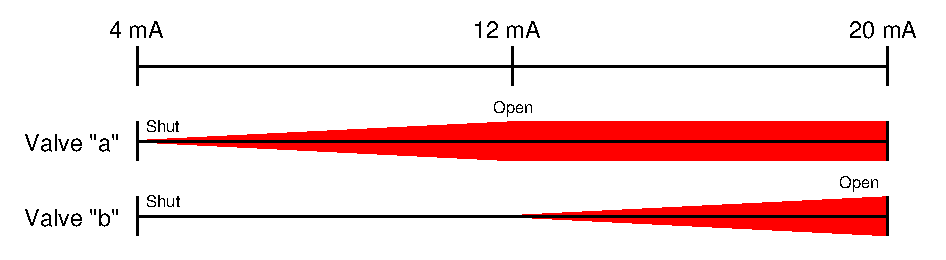
\includegraphics[width=15.5cm]{i00063x01.eps}$$

Vi kan sette opp $y = mx + b$-formler for begge ventiler innenfor omradene de opererer ved a skissere grafer som viser apning \% versus milliamp-signalverdier slik:

$$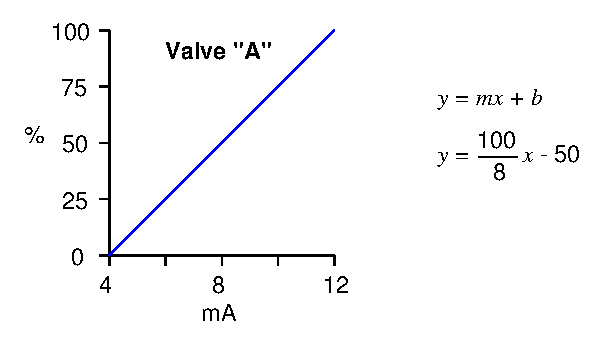
\includegraphics[width=15.5cm]{i00063x02.eps}$$

$$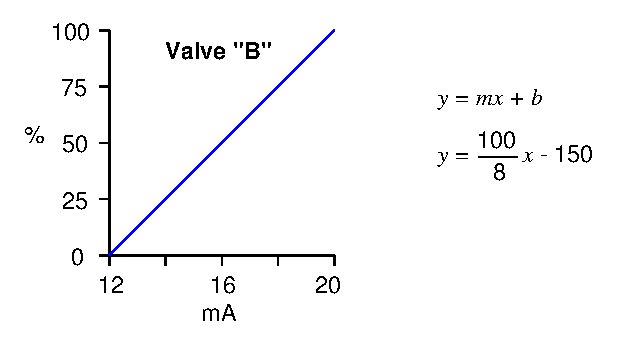
\includegraphics[width=15.5cm]{i00063x03.eps}$$

\vskip 10pt

Ved 6.34 mA: Ventil A = \underbar{\bf 29.25\% apen} \hskip 50pt Ventil B = \underbar{\bf Helt lukket}

\vskip 10pt

Ved 15.81 mA: Ventil A = \underbar{\bf 100\% apen} \hskip 50pt Ventil B = \underbar{\bf 47.63\% apen}


%INDEX% Final Control Elements, valve: split-ranging

%(END_NOTES)


